%---------------------------------------------------------------------------------------------------------------------------
% Kopf des Vortrags
%---------------------------------------------------------------------------------------------------------------------------

\part{Induktive Sensoren}
\begin{center}
Ulf Schmelzer (ulscit01@hs-esslingen.de) \\
Antonio Parrotta (anpait00@hs-esslingen.de)\\[1cm]
26. Oktober 2015 \\[1cm]
\end{center}


%---------------------------------------------------------------------------------------------------------------------------
% Textteil
%---------------------------------------------------------------------------------------------------------------------------
\section*{Einf�hrung}
%\label{Kap_Einf�hrung}

Induktive Sensoren werden in der Industrie eingesetzt, um ferromagnetische Materialien zu detektieren. Dieser Bericht befasst sich mit dessen Entstehung, Funktionsweise, dem Einsatzgebiet und dessen Eigenschaften.

%%%%%%%%%%%%%%%%%%%%%%%%%%%%%%%%%%%%%%%%%%%%%%%%%%%%%%%%%%%%%%%%%%%%%%%%%%%%%%%

\section*{Geschichte}
\label{geschichte}

Die Firma BASF beauftragte im Jahre 1958 das Unternehmen �Pepperl und Fuchs� in Mannheim, eine Alternative zu den bisher eingesetzten mechanischen Schaltern in der Automatisierung zu entwickeln. Die Vorgabe war, dass die Neuentwicklung mehrere tausende Schaltvorg�nge im chemischen Umfeld �berstehen muss, im Gegensatz zu den mechanischen Schaltern, die durch die Gase und Mittel schnell verschlissen.

Zu Beginn der Entwicklung wurden Bipolar-Transistoren verwendet, welche eine einfache Auswertung von
Schwingkreisen und Umwandlung in Schaltsignale erm�glicht haben. Durch den schnellen Wachstum im
Maschinenbau konnte parallel auch der induktive Sensor weiterentwickelt werden. Im Jahre 1968
entstand eine induktive Ausf�hrung des Rollenhebel-Endschalters nach DIN 43 694. Dieser hatte f�nf
verschiedene Seiten f�r die Sensorfl�che, damit alle m�glichen Anfahrrichtungen des mechanischen
Pendant nachempfunden werden konnten. Mittlerweile haben die induktiven N�herungsschalter
gr��tenteils die mechanischen Schalter abgel�st.\cite{geschichte}

%%%%%%%%%%%%%%%%%%%%%%%%%%%%%%%%%%%%%%%%%%%%%%%%%%%%%%%%%%%%%%%%%%%%%%%%%%%%%%%
\section*{Funktionsweise}
\label{funktionsweise}

Mit Hilfe eines LC-Schwingkreises wird ein elektromagnetisches Wechselfeld mit einer Frequenz zwischen 100 $kHz$ und 1 $MHz$ erzeugt. Durch den Einsatz eines hoch permeablen Ferritmaterials kann dem entstehenden Magnetfeld in der Spule eine Vorzugsrichtung gegeben werden. Mit Hilfe eines Ferritkern kann das Feld auf den zu �berwachenden Bereich des Sensors abgestimmt werden.

Wird nun in das erzeugte und gerichtete Magnetfeld das so genannte �Target� (das zu erkennende Ziel) eingebracht, wird nach dem Induktionsgesetz, wie bei einem Transformator, dem Schwingkreis Energie entzogen. Siehe Abbildung \ref{fig:ersatz}.
Dabei kann die Spule des LC-Schwingkreises als Prim�rwicklung und das �Target� als Sekund�rwicklung mit Widerstand als Verbraucher dargestellt werden.

\begin{figure}[h]
	\centering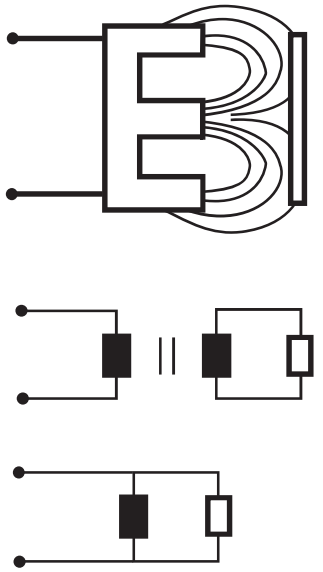
\includegraphics[width=.2\textwidth]{induktiv_sensoren/ersatzschaltbild.png}
	\caption{Ersatzschaltbild eines \\Targets im Magnetfeld\cite{ifm}}
	\label{fig:ersatz}
\end{figure}

Die nun auftretenden Wirbelstromverluste sind von mehreren Faktoren abh�ngig.\cite{ifm}

\begin{itemize}
	\item Abstand und Lage des Gegenstandes vor dem N�herungsschalter 
	\item Abmessungen des Gegenstandes und seiner �u�eren Form 
	\item elektrische Leitf�higkeit und seiner Permeabilit�t.
\end{itemize}

\begin{figure}[h]
	\centering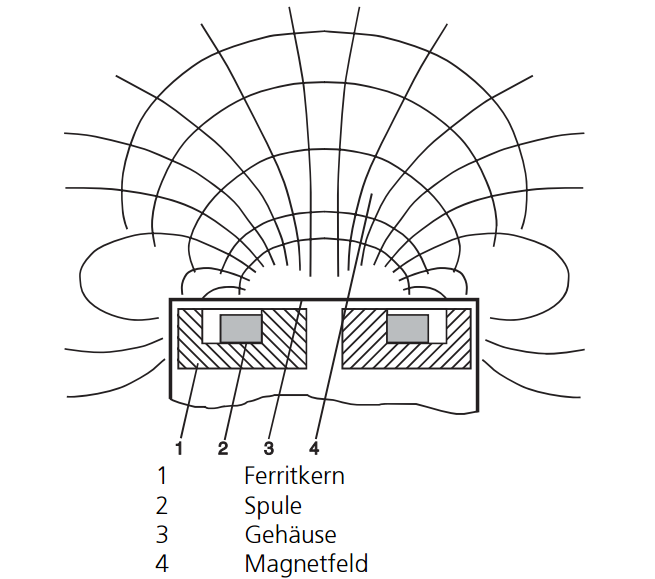
\includegraphics[width=.4\textwidth]{induktiv_sensoren/magnetfeld_sensor.png}
	\caption{Magnetfeld eines induktiven Sensors\cite{ifm}}
	\label{fig:magnetfeld}
\end{figure}

Das nun entstehende ged�mpfte Signal kann mit Hilfe eines Operationsverst�rkers ausgewertet werden, um ein bin�res Signal zu erzeugen. In der Realit�t wird das Signal meistens noch weiter ausgewertet, um z.\,B. Flattern, wenn sich ein Gegenstand sehr langsam n�hert, oder ein fehlerhaftes Schalten beim Anlegen der Betriebsspannung und w�hrend des Einschwingen des LC-Schwingkreises, zu verhindern. Abbildung \ref{fig:prozesskette} veranschaulicht die Prozesskette des induktiven Sensors als Blockschaltbild. 
\vspace{.5cm}
\begin{figure}[h]
	\centering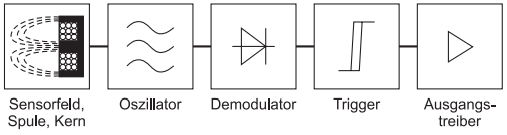
\includegraphics[width=.45\textwidth]{induktiv_sensoren/prozesskette_sensor}
	\caption{Prozesskette eines induktiven Sensors\cite{ifm}}
	\label{fig:prozesskette}
\end{figure}

%%%%%%%%%%%%%%%%%%%%%%%%%%%%%%%%%%%%%%%%%%%%%%%%%%%%%%%%%%%%%%%%%%%%%%%%%%%%%%%
%------------------------------------------------------------------------------------------------------------------------
\section*{Analog Sensor}
\label{analogsensor}
Bei analogen Sensoren wird das entstehende Signal ausgewertet und z.\,B. mit Hilfe eines Microcontrollers vorverarbeitet oder als Analogwert im Bereich von 4-20 $mA$ zur�ckgeliefert. Dieses Signal kann z.\,B. zur Abstandsmessung genutzt werden. Dabei muss allerdings darauf geachtet werden, dass sich das n�hernde Objekt immer auf der selben Bahn und Winkel befindet und auch das Material immer dasselbe ist, da diese Parameter alle in die Wirbelstromverluste einflie�en, was zu stark variierenden Messergebnissen f�hren kann.
Aufgrund dieser Problematik werden Induktivsensoren eher selten zur Abstandsmessung eingesetzt.

\section*{Berechnungen}

\begin{align}
	L=\frac{N^2}{R_m}
\end{align}

\begin{itemize}
	\item $L = $ Induktivit�t
	\item $R_m = $ Widerstand des magnetischen Kreises
	\item $N = $ Windungszahl
\end{itemize}

Der magnetische Widerstand $R_m$ errechnet sich wie folgt:
\begin{align}
	R_m =\frac{l}{\mu_0 \cdot \mu_r \cdot A}
\end{align}

\begin{itemize}
	\item $\mu_0= $ Feldkonstante $1,257 * 10^{-6}\frac{Vs}{Am}$
	\item $\mu_r = $ Permeabilit�tszahl
\end{itemize}

\section*{Ausblick}
%\label{Kap_Fazit}

Obwohl es induktive Sensoren eine ganze Weile gibt, ist das Potenzial ihrer Weiterentwicklung noch nicht erreicht. Es besteht ein Trend in Richtung miniaturisierter, leistungsf�higer Sensorik, sowie in die I/O-Link Technik. Dadurch wird die M�glichkeit geschaffen, induktive Sensoren von der Steuerung aus zu parametrieren. Mit dieser Eigenschaft ist es m�glich, neue Wege der Diagnosefunktionen zu nutzen. Obwohl es noch viel Spielraum f�r Weiterentwicklungen gibt, d�rfen einige Aspekte nicht vernachl�ssigt werden\cite{trend}:

\begin{itemize}
	\item Temperaturabh�ngigkeit
	\item Performance
	\item Schaltabstand
	\item Schaltfrequenz
	\item Kosten
\end{itemize}


%%%%%%%%%%%%%%%%%%%%%%%%%%%%%%%%%%%%%%%%%%%%%%%%%%%%%%%%%%%%%%%%%%%%%%%%%%%%%%%

\begin{thebibliography}{}
%\addcontentsline{toc}{section}{Literatur}
\bibitem{geschichte}
Process.Vogel:\textit{"'Vergangenheit und Zukunft des induktiven N�herungsschalters"'},\\
\href{http://www.process.vogel.de/automatisierung_prozessleittechnik/articles/145538/}{http://www.process.vogel.de/automatisierung\\\_prozessleittechnik/articles/145538/}, \\Aufrufdatum: 30.09.2015

\bibitem{ifm}
IFM:\textit{"'Schulungsunterlagen Induktive Sensoren"'}, \href{http://www.seo-analyse.com/seo-lexikon/e/entwicklungsstadium}{http://www.ifm.com/obj/S100d.pdf},\\
Aufrufdatum: 30.09.2015

\bibitem{trend}
A\&D24: \textit{"'Untersch�tzt: INDUKTIVE SENSOREN"'},\\
\href{http://www.aud24.net/pi/index.php?StoryID=189\&articleID=188851}{http://www.aud24.net/pi/index.php?StoryID=189\\\&articleID=188851},\\
Aufrufdatum: 07.08.2015
\end{thebibliography}
%%%%%%%%%%%%%%%%%%%%%%%%%%%%%%%%%%%%%%%%%%%%%%%%%%%%%%%%%%%%%%%%%%%%%%%%%%%%%%%
